
\subsection{Participants}
The recruitment of 50 L1 Italian L2 English speakers was managed through Prolific \citep{Palan_2018}. For the purposes of this study, we did not ask about 'native status' \citep{Brown_Tusmagambet_Rahming_Tu_DeSalvo_Wiener_2023}; instead we define an L1 Italian speaker as someone who self-identified via Prolific as a fluent Italian speaker, whose first and primary language is Italian. Because Italian is spoken all over the world and we wanted to make a direct comparison to \cite{Sulpizio_McQueen_2012}'s results, we further specified that the participants must be born in Italy. Although not stated in \cite{Sulpizio_McQueen_2012}, we assume all of their participants were fluent in English given that they were university students. Similarly, all of our participants also reported fluency in English as an L2. All participants were required to score an 80\% or higher on the LexITA \citep{Amenta2021}, which estimates Italian vocabulary size and was presented entirely in Italian (and thus requiring participants to be able to read and understand Italian). Three additional participants were removed for LexITA scores below 80\% accuracy. An additional 25 were removed for failed headphone-checks \citep{milne_2021} and/or failed web-camera-checks. To ensure data quality and maximize retained participants, three median absolute deviations (MAD) from median square root transformed reaction time was calculated as the standard for removal for battery tasks \citep{Leys_2013}. Three were removed for being below the three MAD \citep{Leys_2013} range in overall speech cue sensitivity. After removal, 47 participants' (age: $\mu$ = 34.5 years, \textit{sd} = 9.6 years) data were retained for analysis. In total, the tasks reported here took participants approximately 30 minutes to complete. All participants were paid for their time. The study was approved by the authors' Institutional Review Board.

\subsection{Materials}

The primary task (2x2 visual world paradigm design) consisted of 28 pairs of trisyllabic words taken from \cite{Sulpizio_McQueen_2012} that were selected as targets and competitor pairs (see Gorilla experiment spreadsheets). The original audio files from \cite{Sulpizio_McQueen_2012}, recorded at 44 kHz (16 bit resolution, mono), were used. The target-competitor pairs were each made up of two high-frequency real words that are segmentally identical for the first two syllables but differing in stress between the first syllable stress (antepenultimate) and the second syllable (penultimate). That is, the word pairs are suprasegmentally contrastive and segmentally identical for the first two syllables but diverged on the third syllable: e.g., CAlamo vs. caLAta. Each set of visual stimuli consisted of a target (e.g., caLAta), a competitor (e.g., CAlamo), and two distractors (e.g., REmoro and reMOto). The distractors were always a target-competitor pairing as well to ensure balanced looks between visual stimuli. That is, a participant could not tell what the correct target-competitor pairing was just by viewing the visual stimuli pairs and simply ignoring the non-segmentally similar items. Comparisons between first and second syllable acoustic measures and can be found in Table \ref{tab:acoustics}, which shows our mean measurements and \cite{Sulpizio_McQueen_2012}'s mean results (note that spectral tilt is presented as a unitless ratio). All syllables were hand-annotated and automation scripts were used to extract acoustic information \citep{qi_textgrid_maker, dicanio_vowel_acoustics}. Aggregate values were calculated by averaging within stress type and syllable for pitch, amplitude, and spectral tilt. However, duration was calculated by averaging the difference between min and max times of each segment in the text\_grid\_extractor.rmd (see our OSF repository for scripts). 


\begin{figure}[H]
  \centering
  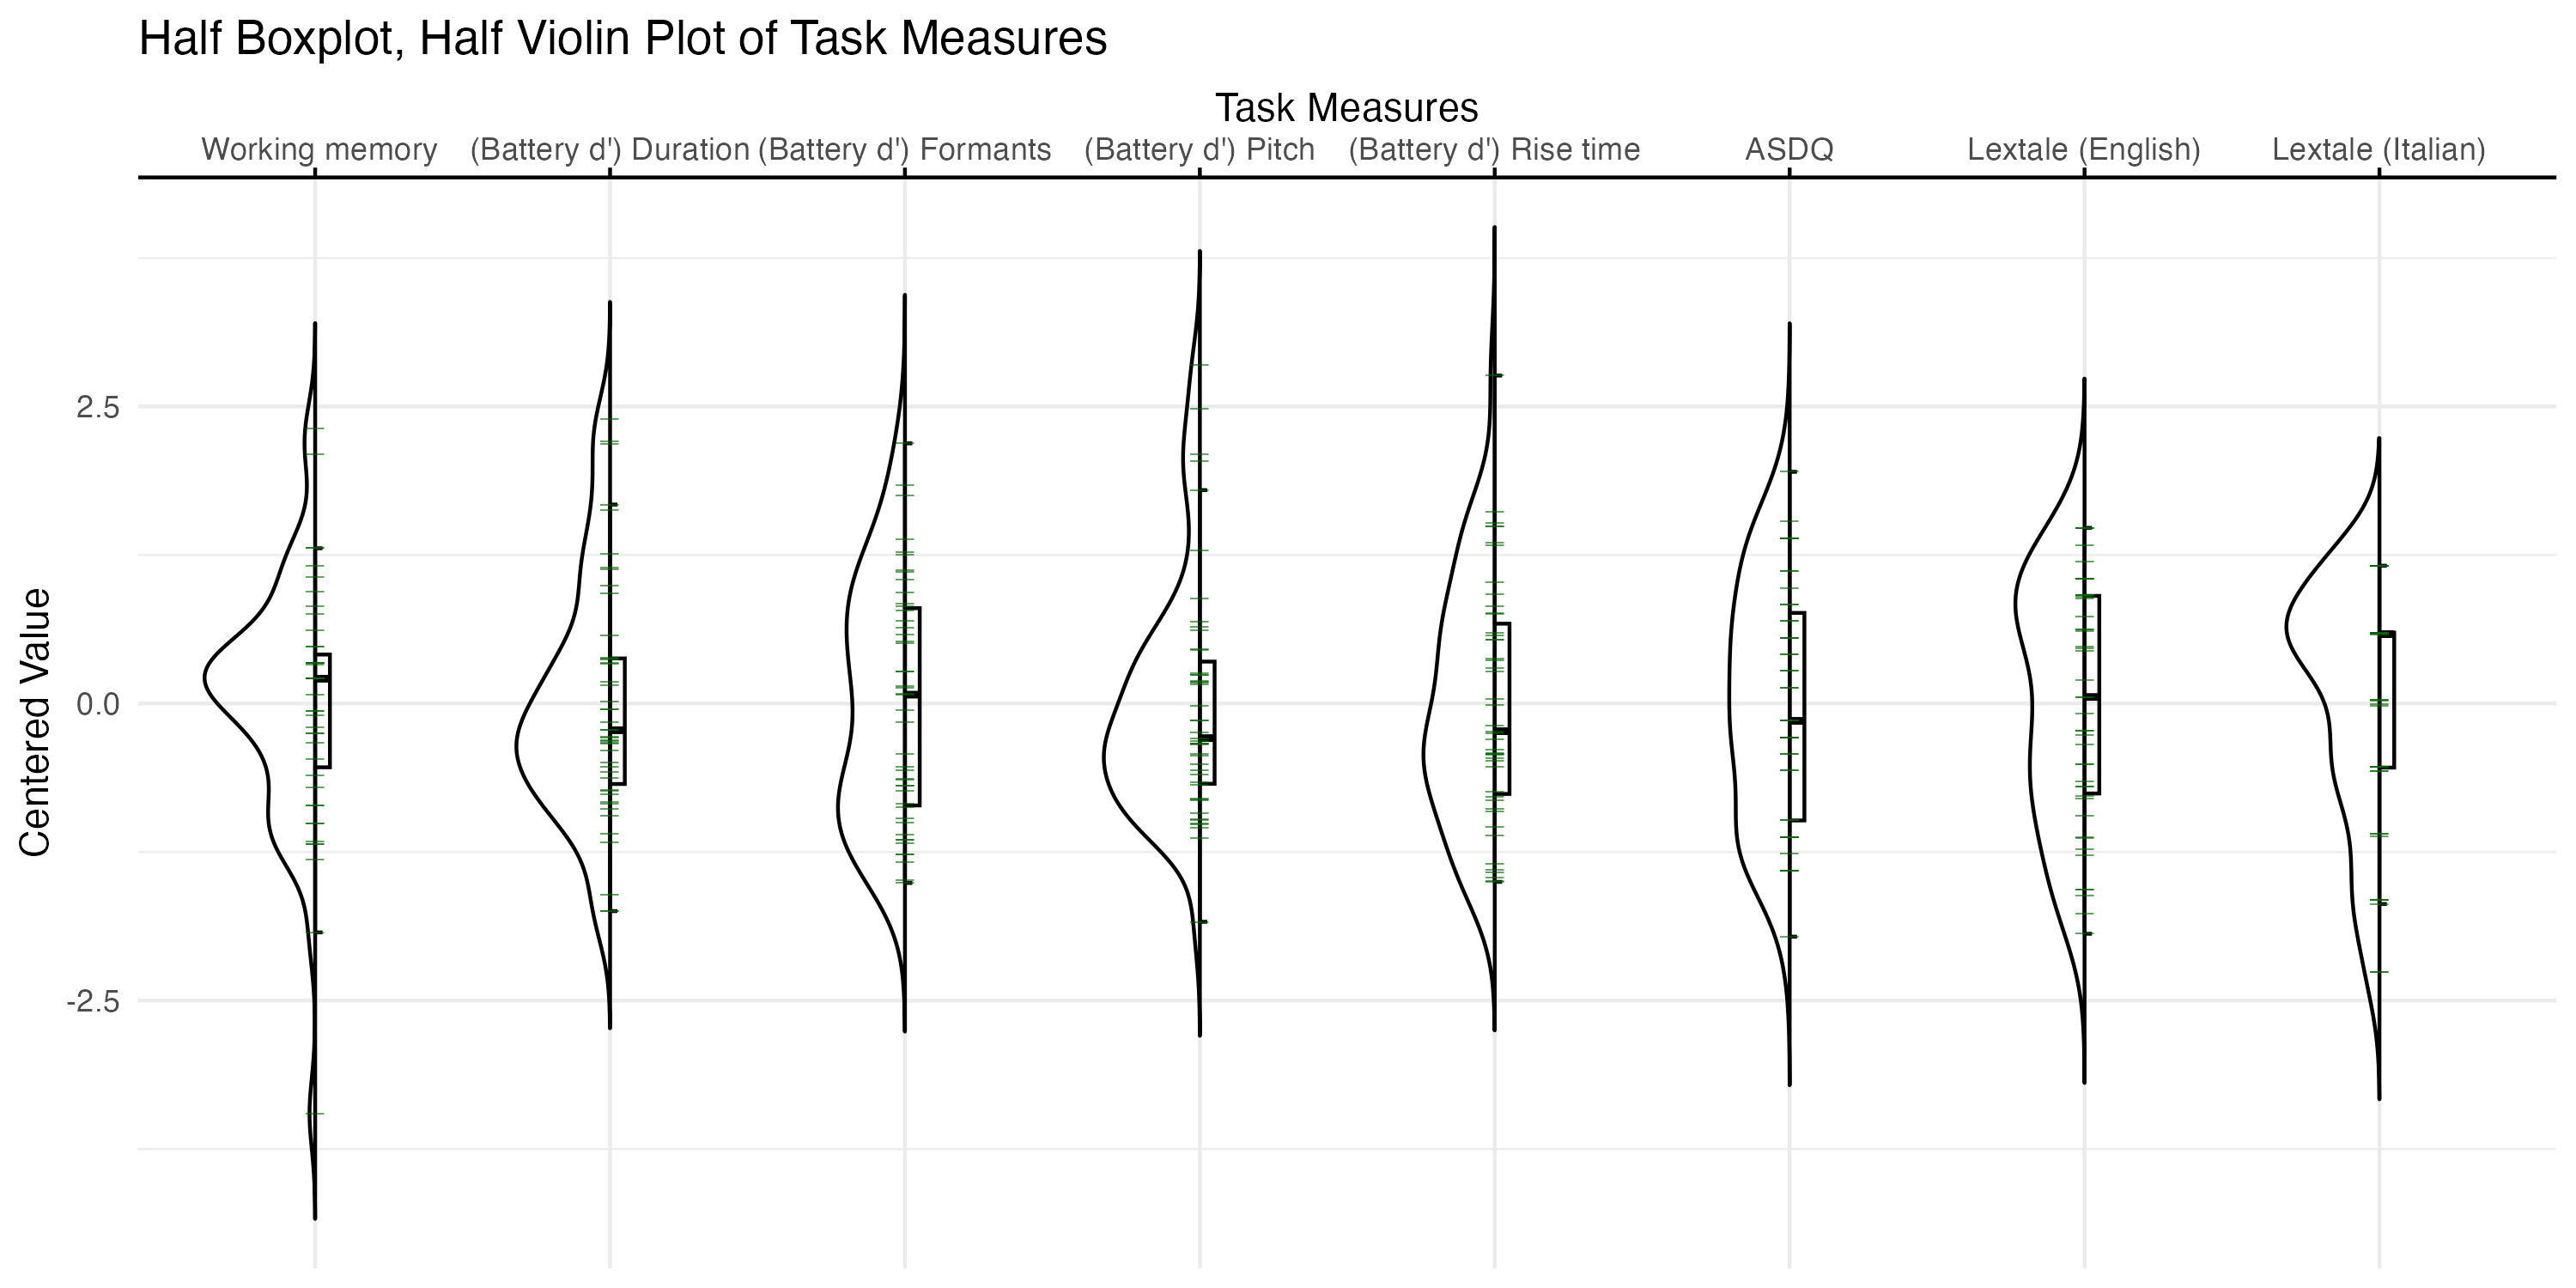
\includegraphics[width=1\linewidth]{visuals/plot_raw_task.jpeg}
  \caption{Centered data across our eight individual difference behavioral tasks.}
  \label{fig:plot_raw_task}
\end{figure}

\begin{table}[ht]
\centering
\caption{Mean acoustic measures for antepenultimate and penultimate first and second syllables}
\begin{tabular*}{\textwidth}{@{\extracolsep{\fill}} lcccccc}
\hline
\textbf{Study} & \textbf{Stress} & \textbf{Cue} & \textbf{1st vowel} & \textbf{2nd vowel} &\textbf{t value} & \textbf{p}\\
\hline
Our study & Antepenultimate & Amplitude (dB)       & .08 & .05 & 7.51  & $<$ .01\\
     &           & Pitch (f0)           & 235 & 182 & 13.17 & $<$ .01\\
     &             & Duration (ms)        & 138 & 71 & 13.11 & $<$ .01\\
     &             & Spectral tilt   & .1 & .09 & 8.26  & $<$ .01 \\
 & Penultimate & Amplitude (dB)      & .09 & .06 & 5.18  & $<$ .01\\
     &             & Pitch (f0)          & 245 & 217 & 6.99  & $<$ .01\\
     &             & Duration (ms)        & 67 & 162 & -20.84 & $<$ .01\\
     &             & Spectral tilt   & .1 & .1 & 0.33  & $>$.05\\
\hline
Sulpizio and &Antepenultimate & Amplitude (dB)    & .09  & .04 & 8.03  & $<$ .01\\
McQueen   &           & Pitch (f0)         & 219 & 177 & 10.54  & $<$ .01\\
 (2012)   &           & Duration (ms)      & 165 & 81  & 16.14  & $<$ .01\\
       &           & Spectral tilt & .7 & .03 & 5.19  & $<$ .01\\
& Penultimate  & Amplitude (dB)     & .09 & .06   & 4.42 & $<$ .01\\
       &           & Pitch (f0)         & 238  & 204 & 4.43 & $<$ .01\\
       &           & Duration (ms)      & 75 & 180   & -18.20 & $<$ .01\\
       &           & Spectral tilt &.3 & .3 & $<$ 1  & $>$.05\\
\hline
\end{tabular*}
\label{tab:acoustics}
\end{table}

\subsection{Procedure}

The experiment was hosted on Gorilla and distributed through Prolific; participants took part on a personal computer in a setting that met the requirements of the experiment, i.e., good lighting and little to no background noise. After consenting, participants were required to do four additional screening tasks: LexITA \cite{Amenta2021}, a basic hearing check which ensured that audio could be heard, a dichotic pitch task \citep{milne_2021} which could only be passed with high quality headphones, and nine-point eye-tracking calibration. If the participants passed all four screenings, the experiment would begin. The remaining experiment consisted of three parts: individual differences tasks, the eye-tracking experiment, and an Italian speech rating task that is part of a different study and not reported here (which was always done last). In total, there were eight individual difference tasks (including LexITA, which was also used to screen participants). Other than the LexITA, all tasks were presented in English. The order of tasks was always fixed, which is shown in Figure \ref{fig:task_structure}. 

\begin{figure}[H]
  \centering
  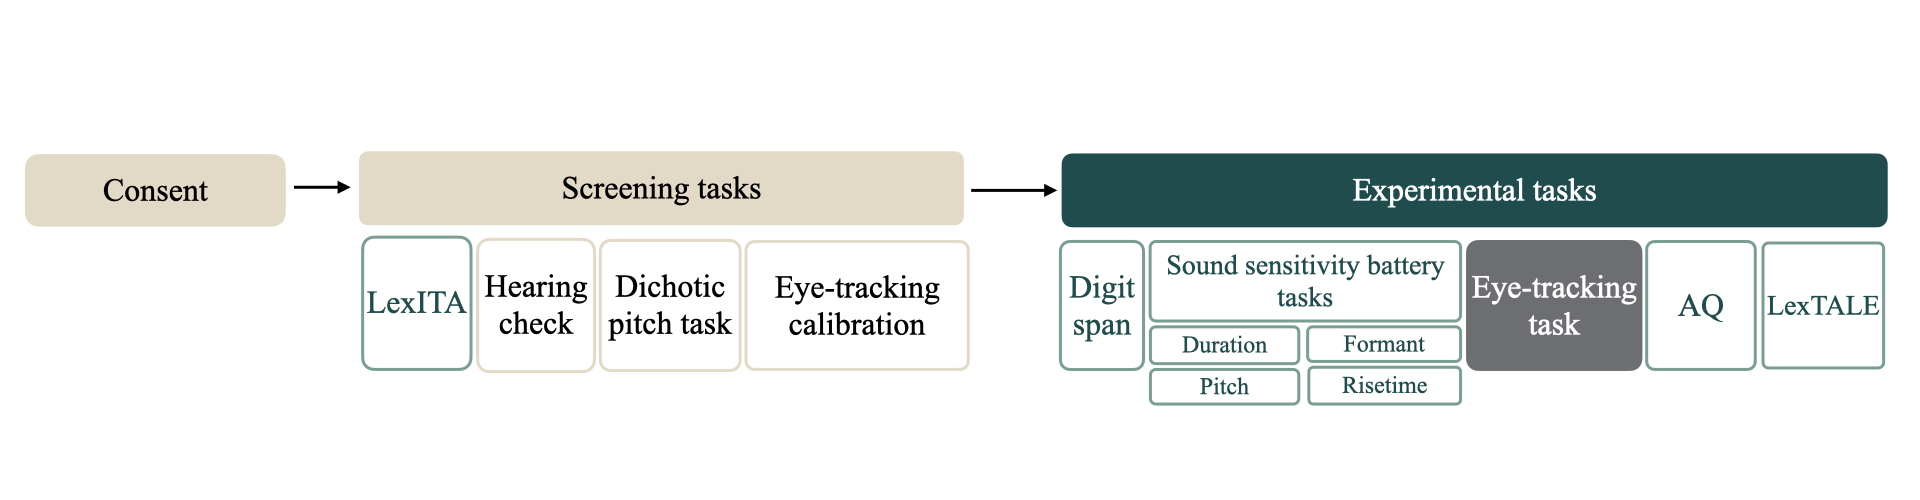
\includegraphics[width=1\linewidth]{visuals/task_structure.jpg}
  \caption{Task structure: All tasks were presented in the same order from beginning (left) to end (right). Note that LexITA is both a measure and a screening task.}
  \label{fig:task_structure}
\end{figure}

LexITA \citep{Amenta2021} consisted of 90 trials (60 real words; 30 non-words). Participants were shown a string of letters and asked to press 'j' if the string of letters was a real word; 'k' if the string was a non-word as quickly and accurately as possible. All instructions were in Italian. A fixation cross was shown for 250 ms between each word. The task took approximately three minutes to complete. The internal consistency for LexITA was .91 as measured by Cronbach's alpha.

After passing the initial four screening tasks, participants began the digit span task. The digit span task presented a series of digits, each displayed for 500 ms and separated by a 250 ms fixation cross. Participants were asked to use their mouse to select the sequence in the same order on a digital number pad. The task began with two digits and had a staircase design with sequence length increasing by one after each correct trial and decreasing by one after each incorrect trial. The task ended after 13 trials. The task took approximately two minutes to complete. The internal consistency for the digit span task was .61 as measured by Cronbach's alpha.

The four battery tasks consisted of AX discrimination tasks which tested participants' sensitivity to pitch, risetime, duration, and formant contrasts; The internal consistency for each type was .54, .85, .72, and .73, respectively as measured by Cronbach's alpha. For each task (36 trials per task), one sound was presented followed by a 250 ms fixation cross and then a second sound. Participants were asked to use the `z' and `m' keys to indicate whether the sounds were the same or different. For all battery tasks, a continuum of 50 stimuli was used \citep{Kachlicka_Saito_Tierney_2019}. 10 of these were selected at various distances (15-55). The distance between stimuli and same/different trials was presented randomly. Each battery task took approximately 90 seconds to complete. It should be noted that the battery tasks and the digit span all have variably difficult items. That is, 2 digits is easier than 9 digits; said another way, lower internally reliability as measured by \citep{Cronbach1951} is reasonable in these tasks given their design. 

For the eye-tracking task, eye-fixations were captured using WebGazer.js \citep{Papoutsaki} implemented in Gorilla \citep{Anwyl-Irvine_2019}. All audio stimuli and word pairings were taken from \cite{Sulpizio_McQueen_2012}. All 64 experimental and distractor words were shown in lower-case letters (font size 20) balanced across the four quadrants across 128 trials. Visual stimuli were placed maximally apart to increase the distance between areas of interest. Distractor and experimental trials were presented in random order. Like \cite{Sulpizio_McQueen_2012}, each trial began with a fixation cross that was displayed for 500 ms. Next, the audio stimuli and visual stimuli were presented simultaneously with the carrier phrase, "Clicca sulla parola" ('click on the word'). After the audio file finished playing ($\mu$ = 110 ms, \textit{sd} = 51 ms), visual stimuli stayed on the screen for 5000 ms (or until the participant clicked on the perceived word). The experiment was preceded by practice trials. Before their experiment, \cite{Sulpizio_McQueen_2012} did a read-aloud familiarization task with the participants, but zero words were unknown to any participant. For this reason (and to shorten the overall experiment length) we decided to remove the familiarization task due to the relatively high frequency of the words. The eye-tracking task took approximately seven minutes to complete.

After completion of the eye-tracking task, participants then took part in the English LexTALE \citep{lemhofer2012introducing} task as well as the autism-spectrum quotient questionnaire (AQ) \citep{Baron-Cohen2001}. Both of these tasks were purposefully put after the eye-tracking task to mitigate negative effects on task performance \citep{Chang_2024}. In the English LexTALE task, participants were shown a fixation cross for 500 ms and then a string of letters was displayed for 2000 ms. Participants were asked to use the keys 'j' and 'k' to decide whether the presented letters formed a real word or non-word within the allotted time \cite{lemhofer2012introducing}. Participants did 60 trials (40 words; 20 non-words), which took approximately three minutes to complete. The LexTale Cronbach’s alpha was .89.  

The AQ \citep{Baron-Cohen2001} consisted of 50 multiple choice questions, each with four options: ``strongly disagree", ``disagree", ``agree", and ``strongly agree". The direction of high tendency scoring was balanced across questions (i.e., ``strongly agree" and ``strongly disagree" were marked as high tendency equally). The 50 questions covered five areas (10 questions per area): social skills, attention switching, attention to detail, communication, imagination. The AQ took approximately five minutes to complete. The internal consistency of the questions, as measured by Cronbach’s alpha was .67.


\subsection{Data analysis}

All analyses were carried out in R \citep[version 4.2.2;][]{R} with a 0.05 alpha level. The individual difference measures were calculated so that each participant had a single score for each task. For the digit span task, each participant's max digit correct was used as a measure of working memory capacity. All reaction times below 200 ms were removed across the four battery tasks as well as the LexITA and LexTALE. For the four battery tasks, hits and false-alarms for each trial were scored and sensitivity to each contrast type was then calculated using d-prime. The scores for both Italian LexITA and English LexTALE are usually calculated by averaging the accuracy of words and non-word to control for bias toward a particular selection choice \citep{lemhofer2012introducing}. However, we calculated both scores by using d$'$ (for both LexITA and LexTALE) after ignoring non-responses, which also controls for bias by using the difference between z-scored hits and false-alarms. A constant of .5 was added to both hits and false-alarms with a Haldane correction/log-linear correction to handle hit and false alarm values of 0 or 1 \citep{Hautus1995}. Lastly, the AQ was scored using Baron-Cohen et al.'s rubric: autistic-like behavior was scored as 1 (irrespective of “slightly” or “definitely” response); non-autistic-like behavior was scored as 0 (irrespective of "slightly" or “definitely” response). Participants were given a total score (0 to 50); scores of 32 or greater represented what Baron-Cohen et al. call “a useful cutoff for distinguishing individuals who have clinically significant levels of autistic traits” (2001, 15). 

For eye-tracking data removal, eye-fixations outside the possible screen area were removed. As suggested in \cite{bramlett_wiener_24-AOW}, quadrants were defined by the origin to maximize signal retention. Fixations at the beginning of the trials were normally distributed from the center at the beginning trials along both the x and y axes. Eye-fixations with face confirmation below 50\% certainty were removed. We retained approximately 96.14\% of eye-fixations (3.86\% data loss). Unlike other recent online web-based eye-tracking experiments we did not remove any data for low frame rate. We set a minimal frame rate for participants to 5 fps \citep{Vos_2017}. However, no participants qualified for removal based on their median frame rate. 


